\documentclass[titlepage, 11pt]{article}

\oddsidemargin=17pt \evensidemargin=17pt
\headheight=9pt     \topmargin=26pt
\textheight=564pt   \textwidth=433.8pt

\usepackage{url}
\usepackage{listings}
\usepackage[pass]{geometry}
% \usepackage{vmargin}
\usepackage{fancyhdr}
\usepackage{amsmath}
\usepackage{amsfonts,amssymb,amsthm,cite,float,graphicx}
% \usepackage[tight,footnotesize]{subfigure}
\usepackage[usenames]{color}
\usepackage{algorithm,algorithmic}
\usepackage{natbib}    % this package seems sensitive to location placement
\usepackage{graphicx}
\usepackage{caption}
\usepackage{subcaption}
\usepackage{multicol}
\usepackage{float}
\usepackage{mathtools}

\newcommand{\excise}[1]{}
\newcommand{\comment}[1]{{$\star$\sf\textbf{#1}$\star$}}

\leftmargini=5.5ex
\leftmarginii=3.5ex

%new math symbols taking no arguments
\newcommand\0{\mathbf{0}}
\newcommand\CC{\mathbb{C}}
\newcommand\FF{\mathbb{F}}
\newcommand\NN{\mathbb{N}}
\newcommand\QQ{\mathbb{Q}}
\newcommand\RR{\mathbb{R}}
\newcommand\ZZ{\mathbb{Z}}
\newcommand\bb{\mathbf{b}}
\newcommand\kk{\Bbbk}
\newcommand\mm{\mathfrak{m}}
\newcommand\pp{\mathfrak{p}}
\newcommand\xx{\mathbf{x}}
\newcommand\yy{\mathbf{y}}
\newcommand\GL{\mathit{GL}}
\newcommand\into{\hookrightarrow}
\newcommand\nsub{\trianglelefteq}
\newcommand\onto{\twoheadrightarrow}
\newcommand\minus{\smallsetminus}
\newcommand\goesto{\rightsquigarrow}
\newcommand\nsubneq{\vartriangleleft}

%redefined math symbols taking no arguments
\newcommand\<{\langle}
\renewcommand\>{\rangle}
\renewcommand\iff{\Leftrightarrow}
\renewcommand\phi{\varphi}
\renewcommand\implies{\Rightarrow}

%new math symbols taking arguments
\newcommand\ol[1]{{\overline{#1}}}

%redefined math symbols taking arguments
\renewcommand\mod[1]{\ (\mathrm{mod}\ #1)}

%roman font math operators
\DeclareMathOperator\aut{Aut}

%for easy 2 x 2 matrices
\newcommand\twobytwo[1]{\left[\begin{array}{@{}cc@{}}#1\end{array}\right]}

%for easy column vectors of size 2
\newcommand\tworow[1]{\left[\begin{array}{@{}c@{}}#1\end{array}\right]}

   \title{ECE 590: \\\textit{Scalability}}
\author{Faris Sbahi, Andrew Bihl, Xinghao}

\begin{document}
\maketitle

\section{Code Analysis}

We designed our Exchange Engine using Golang. One of the primary motivators for doing so is Go's built-in concurrency system, centered around the use of goroutines. Goroutines are similar to threads, however instead of there existing a one-to-one mapping of threads to goroutines, each goroutine is mapped to a group of threads. Hence, once the swap context and thread setup overhead becomes too high, Go will start mapping parallelized executions to the same threads.

Hence, each time our server accepts a request, the request is handled as part of a separate goroutine. This is our first level of parallelization. 

Furthermore, we parse the received XML as part of a stream which allows us to start performing a job in parallel (e.g. buy order) as we continue reading. This seems especially useful for requests that consist of an extremely large amount of data.

When dealing with "transaction" and "create" requests, idempotency and atomicity become increasingly important because there are several places that a given request can fail. Hence, it was clear that we needed to execute certain operations atomically and rollback if a single command in the operation failed. For example, cancel transactions must both deposit money to a user's account and remove the open shares from the market. The first step of atomicity is solved using a simple mutex. Furthermore, if the shares can't be removed, then the transaction to deposit funds into the user's account is rolled back. We ignore cancel requests for transaction IDs which we've already cancelled. This provides idempotency. 

Still, query transactions don't actually modify data so it seemed like an unecessary overhead to use the same mutex that we use for the other transactions. Hence, we decided to measure the effect a Reader-Writer Lock (RWMutex in Go) would have on our scalability. From the docs, if a goroutine holds a RWMutex for reading and another goroutine might call Lock, no goroutine should expect to be able to acquire a read lock until the initial read lock is released.

Another important consideration is the datastore. Our initial design simply used a hashmap, which provided great speed given that data would tend to reside in memory. We recognized that we needed some sort of database so that the server can go down without transaction history being permanently deleted. Our first choice was Postgres . Later, we wondered if we could recover the benefits we saw when we used a dictonary. Hence, we explored the possibility of using Redis as an in-memory cache. In our experiments below, we explore the effect it had on our scalability.

\section{Experiments}

% Explain methodology e.g. how we timed things

\subsection{Scalability}

As mentioned in our code analysis, it was left to measure whether Reader-Writer Locks substantially improved our performance. One simple test was to send 1000 requests in parallel that are reader-intensive 

\begin{lstlisting}
time seq 1000 | parallel -n0 "cat transaction/query/1.txt | nc localhost 12345"
\end{lstlisting}

Average over 10 experiments, we found that the RWMutex method took 15.191s, substantially better than 19.463s found using regular mutexes.

WE NEED A LOT OF CHARTS HERE

I INCLUDED ONE OF HILTON'S CHARTS BELOW

\begin{figure}[H]
\centering
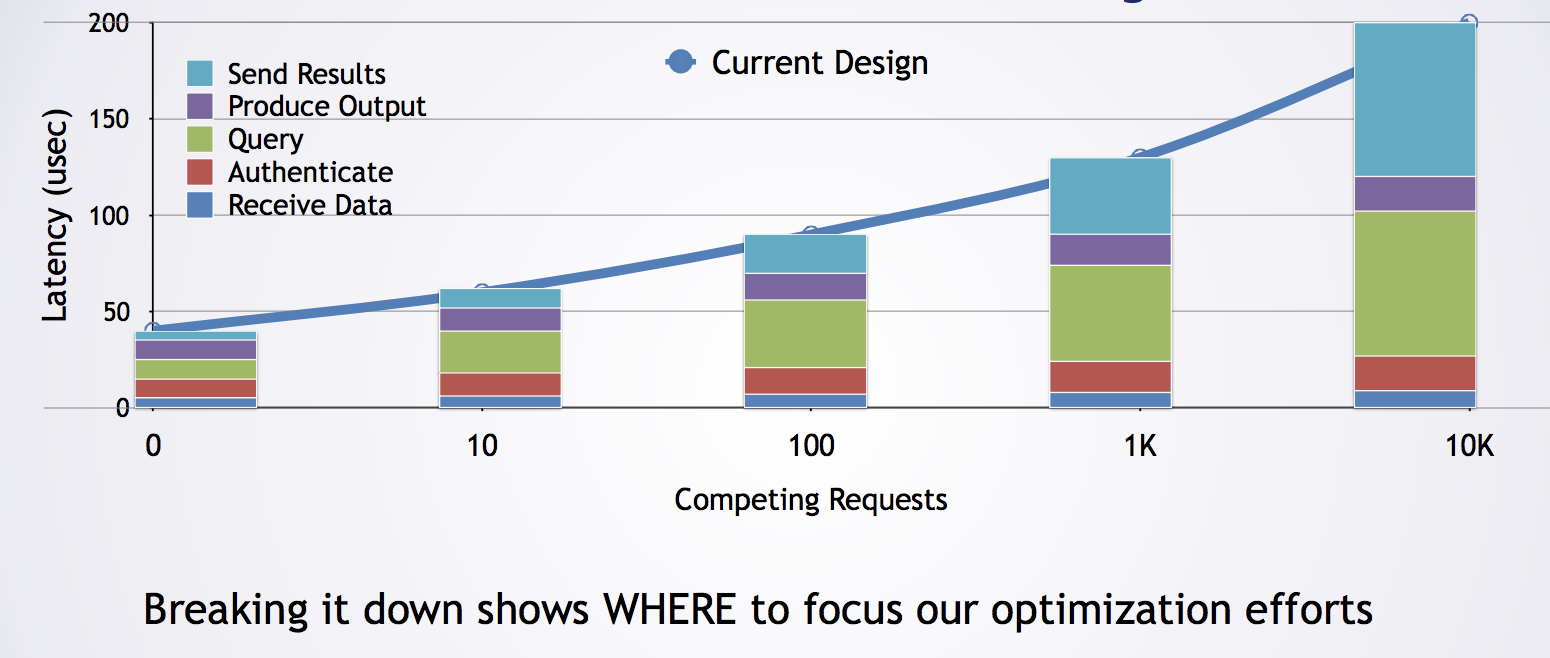
\includegraphics[width=\linewidth]{sample_hilton.png}	
\caption{Scalability Breakdown}
\end{figure}

EXPLAIN HOW WE GOT THIS DATA EXPERIMENTALLY

\subsection{Correctness}

We developed specialized test cases that are executed as part of our \texttt{tests.sh} script. These ensure that we have correctness for the standard and edge cases that we came up with. Furthermore, we dump the database as part of our separate debug log each time we handle a request. Hence, we are able to see whether the correct values exist in the database at each step. 

Furthermore, we tested for datastore failures my taking down the Redis and Postgres containers and random points of our testing and ensured that the same results were achieved. 

\section{Discussion}

Evidently, we found that using Redis as a cache seriously improved our ability to scale. 

Furthermore, we found that INSERT is our greatest bottleneck. One way we could mitigate this, if we were to continue working on this project is to .... 

\end{document}
